\documentclass[11pt,a4paper]{article}
\usepackage[
    left=0.73in,
    right=0.73in,
    top=.8in,
    bottom=.50in,
    paperheight=11in,
    paperwidth=8.5in
]{geometry}

\usepackage{array}
\newcolumntype{C}[1]{>{\centering\let\newline\\\arraybackslash\hspace{0pt}}m{#1}}

\usepackage{graphicx}
\usepackage{subcaption}

\begin{document}
% Cover Page
\pagenumbering{gobble}
\begin{center}
\textbf{
    \Large{ECE 543: Introduction to Digital Systems}
    \\~\\
    \large{Instructor: Bessam Zuhair Al Jewad, Ph.D.}
    \\[1.25in]
    \LARGE{Prelab \#2: Introduction to integrated circuits and data books}
    \\[0.62in]
    \large{Prepared for Himadri Basu (TA)\\~\\By Christopher Chin}
    \\[1.25in]
    \LARGE{Section 6}
    \\[1.25in]
    \Large{Department of Electrical and Computer Engineering\\
           University of New Hampshire}
    \\[1.25in]
    \Large{\today}
}
\end{center}
\clearpage
\pagenumbering{arabic}

% TOC
\tableofcontents
\pagebreak

% Pages
\section{Introduction}
The objective of this experiment is to become more familiar with TTL integrated
circuits and the data sheets which describe their electrical characteristics.
\section{Equipment Required}
\begin{itemize}
    \item Global Specialties Design and Prototyping PB-505
    \item Wire Leads
    \item Unknown TTL Integrated Circuit (1)
\end{itemize}
\section{Procedure}
\subsection{IC Diagrams}
\begin{figure}[h]
    \begin{subfigure}{.3\textwidth}
        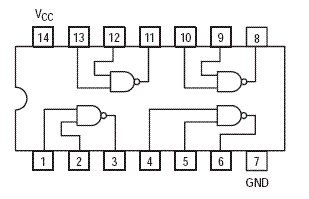
\includegraphics[width=2in]{IC7400.png}
        \caption{IC7400 Circuit Diagram}
    \end{subfigure}
    \begin{subfigure}{.3\textwidth}
        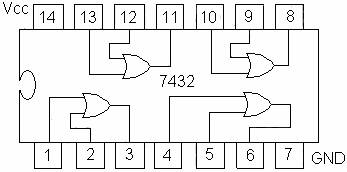
\includegraphics[width=2in]{IC7432.png}
        \caption{IC7432 Circuit Diagram}
    \end{subfigure}
    \begin{subfigure}{.3\textwidth}
        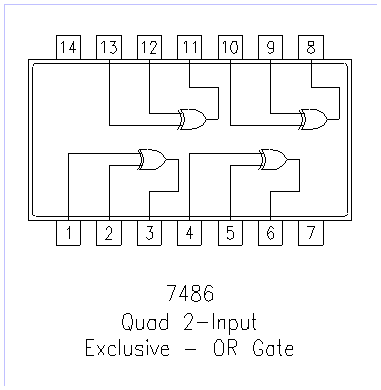
\includegraphics[width=2in]{IC7486.png}
        \caption{IC7486 Circuit Diagram}
    \end{subfigure}
\end{figure}
Each IC has the same internal connections.
Pin 14 is used as VCC$_{in}$. Pin 7 is GND.
Pin 1 and 2 are inputs to a logic gate that outputs to pin 3.
Pin 4 and 5 are inputs to a logic gate that outputs to pin 6.
Pin 13 and 12 are inputs to a logic gate that outputs to pin 11.
Pin 10 and 9 are inputs to a logic gate that outputs to pin 8.
For IC7400 all the internal logic gates are NAND gates.
For IC7432 all the internal logic gates are OR gates.
For IC7486 all the internal logic gates are XOR gates.

\subsection{Logic Tables}
Assume Pins 1, 2, 4, and 5 are inputs controlled by S3, S2, S1, S0 respectively.
\\[.5in]
\captionof{table}{IC7400 Logic Table}
\begin{tabular}{| C{1.83cm} | C{1.83cm} | C{1.83cm} | C{1.83cm} | C{1.83cm} | C{1.83cm} | C{1.83cm} | }
    \hline
        \multicolumn{4}{|c|}{Inputs}
        & \multicolumn{2}{|c|}{Intermediates}
        & Output \\
    \hline
        S3 & S2 & S1 & S0 & Pin 3 & Pin 6 & Logic Monitor, 0 \\
    \hline
        0  & 0  &  0 &  0 & 1 & 1 & 0\\
    \hline
        0  & 0  &  0 &  1 & 1 & 1 & 0\\
    \hline
        0  & 0  &  1 &  0 & 1 & 1 & 0\\
    \hline
        0  & 0  &  1 &  1 & 1 & 0 & 1\\
    \hline
        0  & 1  &  0 &  0 & 1 & 1 & 0\\
    \hline
        0  & 1  &  0 &  1 & 1 & 1 & 0\\
    \hline
        0  & 1  &  1 &  0 & 1 & 1 & 0\\
    \hline
        0  & 1  &  1 &  1 & 1 & 0 & 1\\
    \hline
        1  & 0  &  0 &  0 & 1 & 1 & 0\\
    \hline
        1  & 0  &  0 &  1 & 1 & 1 & 0\\
    \hline
        1  & 0  &  1 &  0 & 1 & 1 & 0\\
    \hline
        1  & 0  &  1 &  1 & 1 & 0 & 1\\
    \hline
        1  & 1  &  0 &  0 & 0 & 1 & 1\\
    \hline
        1  & 1  &  0 &  1 & 0 & 1 & 1\\
    \hline
        1  & 1  &  1 &  0 & 0 & 1 & 1\\
    \hline
        1  & 1  &  1 &  1 & 0 & 0 & 1\\
    \hline
\end{tabular}

\captionof{table}{IC7432 Logic Table}
\begin{tabular}{| C{1.83cm} | C{1.83cm} | C{1.83cm} | C{1.83cm} | C{1.83cm} | C{1.83cm} | C{1.83cm} | }
    \hline
        \multicolumn{4}{|c|}{Inputs}
        & \multicolumn{2}{|c|}{Intermediates}
        & Output \\
    \hline
        S3 & S2 & S1 & S0 & Pin 3 & Pin 6 & Logic Monitor, 0 \\
    \hline
        0  & 0  &  0 &  0 & 0 & 0 & 0\\
    \hline
        0  & 0  &  0 &  1 & 0 & 1 & 1\\
    \hline
        0  & 0  &  1 &  0 & 0 & 1 & 1\\
    \hline
        0  & 0  &  1 &  1 & 0 & 1 & 1\\
    \hline
        0  & 1  &  0 &  0 & 1 & 0 & 1\\
    \hline
        0  & 1  &  0 &  1 & 1 & 1 & 1\\
    \hline
        0  & 1  &  1 &  0 & 1 & 1 & 1\\
    \hline
        0  & 1  &  1 &  1 & 1 & 1 & 1\\
    \hline
        1  & 0  &  0 &  0 & 1 & 0 & 1\\
    \hline
        1  & 0  &  0 &  1 & 1 & 1 & 1\\
    \hline
        1  & 0  &  1 &  0 & 1 & 1 & 1\\
    \hline
        1  & 0  &  1 &  1 & 1 & 1 & 1\\
    \hline
        1  & 1  &  0 &  0 & 1 & 0 & 1\\
    \hline
        1  & 1  &  0 &  1 & 1 & 1 & 1\\
    \hline
        1  & 1  &  1 &  0 & 1 & 1 & 1\\
    \hline
        1  & 1  &  1 &  1 & 1 & 1 & 1\\
    \hline
\end{tabular}

\captionof{table}{IC7486 Logic Table}
\begin{tabular}{| C{1.83cm} | C{1.83cm} | C{1.83cm} | C{1.83cm} | C{1.83cm} | C{1.83cm} | C{1.83cm} | }
    \hline
        \multicolumn{4}{|c|}{Inputs}
        & \multicolumn{2}{|c|}{Intermediates}
        & Output \\
    \hline
        S3 & S2 & S1 & S0 & Pin 3 & Pin 6 & Logic Monitor, 0 \\
    \hline
        0  & 0  &  0 &  0 & 0 & 0 & 0\\
    \hline
        0  & 0  &  0 &  1 & 0 & 1 & 1\\
    \hline
        0  & 0  &  1 &  0 & 0 & 1 & 1\\
    \hline
        0  & 0  &  1 &  1 & 0 & 0 & 0\\
    \hline
        0  & 1  &  0 &  0 & 1 & 0 & 1\\
    \hline
        0  & 1  &  0 &  1 & 1 & 1 & 0\\
    \hline
        0  & 1  &  1 &  0 & 1 & 1 & 0\\
    \hline
        0  & 1  &  1 &  1 & 1 & 0 & 1\\
    \hline
        1  & 0  &  0 &  0 & 1 & 0 & 1\\
    \hline
        1  & 0  &  0 &  1 & 1 & 1 & 0\\
    \hline
        1  & 0  &  1 &  0 & 1 & 1 & 0\\
    \hline
        1  & 0  &  1 &  1 & 1 & 0 & 1\\
    \hline
        1  & 1  &  0 &  0 & 0 & 0 & 0\\
    \hline
        1  & 1  &  0 &  1 & 0 & 1 & 1\\
    \hline
        1  & 1  &  1 &  0 & 0 & 1 & 1\\
    \hline
        1  & 1  &  1 &  1 & 0 & 0 & 0\\
    \hline
\end{tabular}
\subsection{Wiring Diagram}
\begin{figure}[h]
    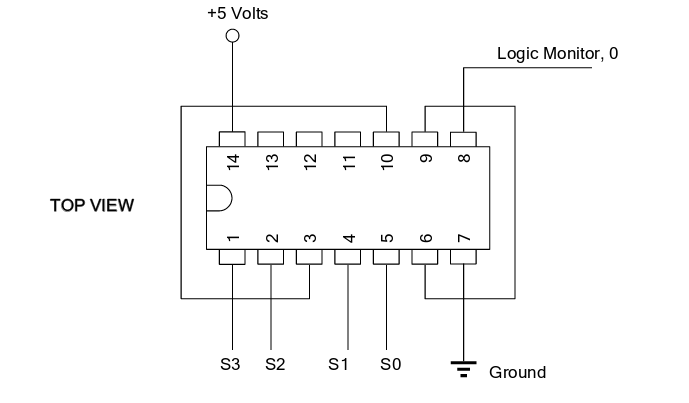
\includegraphics[width=5in]{IC-wires.png}
\end{figure}
This wiring format will be used for each IC.
Pin 14 is used as VCC$_{in}$. Pin 7 is GND.
Pins 1, 2, 4, and 5 will act as input pins controlled by S3, S2, S1, and S0 respectively.
Based on the IC diagrams, pins 1 and 2 will affect pin 3 which will be connected to pin 10.
Based on the IC diagrams, pins 4 and 5 will affect pin 6 which will be connected to pin 10.
Based on the IC diagrams, pins 10 and 9 will affect pin 8 which will be connected to our logic monitor.

\pagebreak
\subsection{Pin Gate relationship}
\begin{figure}[h!]
    \begin{subfigure}{.7\textwidth}
        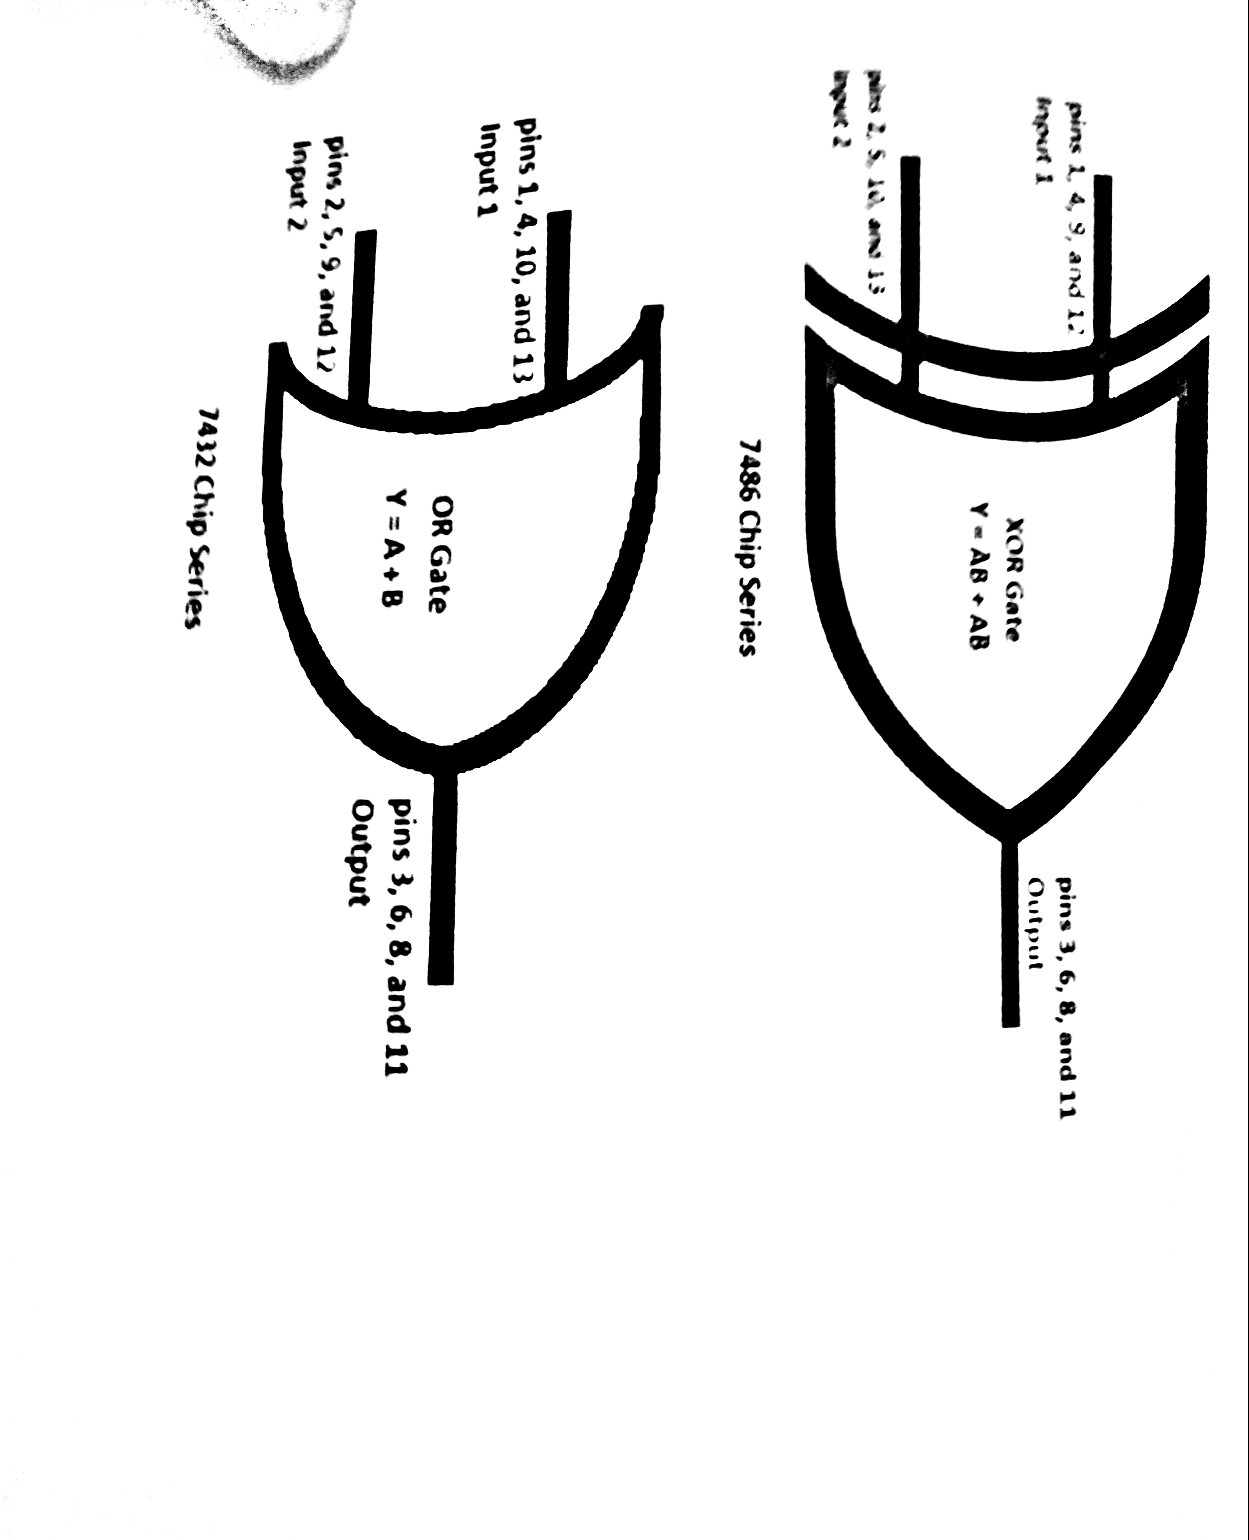
\includegraphics[width=4in]{XOR_OR_gates.jpg}
    \end{subfigure}
    \begin{subfigure}{.3\textwidth}
        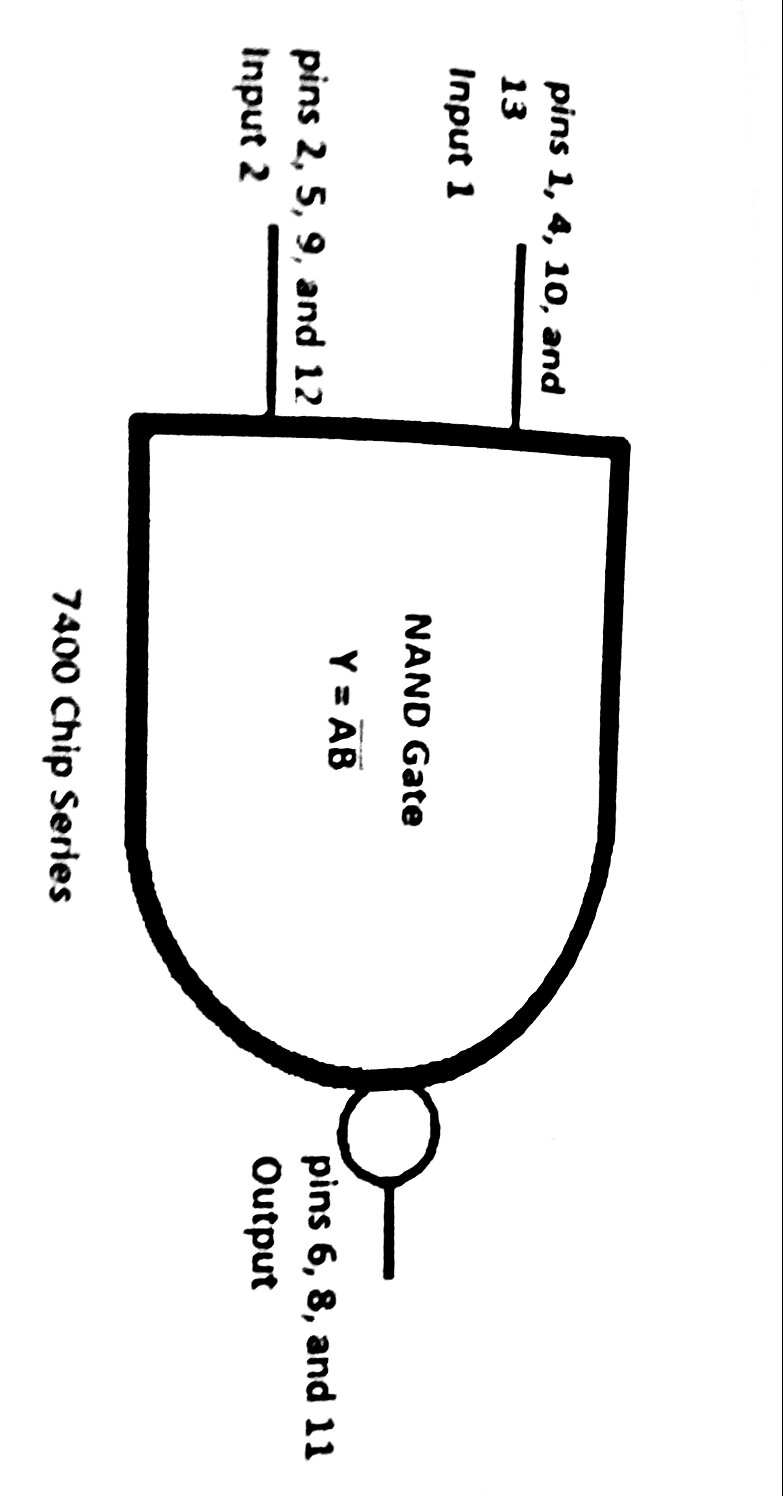
\includegraphics[width=2in]{NAND_gate.jpg}
    \end{subfigure}
\end{figure}

\section{References}
Ronald J. Tocci et al. 2011. Digital Systems: Principles and Applications, 11\textsuperscript{th} Ed.

See these links for datasheets:
https://fairchildsemi.com
https://ti.com
\end{document}
